\section{Technology and setup}
\label{chap:tech}
This section will explain all the components used for the development environment. 
\subsection{Jupyter Notebook}
The model is developed in the form of a \gls{jupyter} \cite{noauthor_project_nodate} using the Python programming language. \gls{jupyter}s are documents that can contain code, text, images, diagrams and explanations. This is especially suitable for this project, because in Machine Learning it is often useful to explain the source code with graphs and diagrams.

\subsection{Google Colaboratory}
The notebook was initially hosted on Google \gls{colab}oratory \cite{colab}. This brought the following advantages:
\paragraph{Synchronization} 
By storing the notebook in a central location, Google Drive, and having everyone access the same notebook, all changes are immediately visible to all users of the notebook.
\paragraph{Project structure} 
The \gls{jupyter} allows to map the whole project in a structured way in a single file. 
\paragraph{Project dependencies}
Since the project is hosted on Google \gls{colab}, it is not necessary as a developer to install libraries and other dependencies locally.

However, as it turned out, \gls{colab} removes from the platform external resources that were imported into the project after a certain time. This meant that I had to re-import the datasets, which are essential for the development of my model, before each work. This forced me to set up a \gls{virtual machine} on which the notebook can then be run locally.

\subsection{Virtual machine}
To have the tools installed in one place, I opted for a virtual machine.
Not only this, the VM has precisely other advantages, which are:
\begin{itemize}
    \item more computing power
    \item do not use my local machine 
    \item is always on, so it can always work
    \item the models are trained on a special machine with special software
    \item being online I can work from any location
    \item always working I can train my models also at night
    \item if by chance something goes wrong, I can backup and create another VM
\end{itemize}

\subsection{Kaggle}
What is Kaggle \cite{noauthor_kaggle_nodate}? 
As it is possible to find written in the documentation: 
\begin{quote}
    "Kaggle is an AirBnB for Data Scientists - this is where they spend their nights and weekends." – Zeeshan-ul-hassan Usmani \cite{zeeshan-ul-hassan_what_2018}
\end{quote}
Founded in 2010 by Anthony Goldbloom (CEO) and Ben Hamner (CTO), and acquired by Google in 2017, Kaggle enables data scientists and other developers to engage in running machine learning contests, write and share code, and to host datasets. 

Kaggle is an online community for data scientists that offers:
\begin{itemize}
    \item machine learning competitions,
    \item datasets,
    \item notebooks,
    \item access to training accelerators,
    \item education.
\end{itemize}
Thanks to its 35k datasets, Kaggle is the perfect place to start a search for a datasets, notebooks or information.

\subsection{Anaconda}
\gls{anaconda} \cite{anaconda_inc_anaconda_nodate} is a distribution of the Python and R programming languages, used for data science, machine learning etc.
\gls{anaconda} is used to simplify package management and deployment of various libraries.
To run \gls{jupyter} with all the needed libraries, \gls{anaconda} has turned out to be a suitable solution. \gls{anaconda} is a platform that allows to set up large projects locally by creating so-called "environments" that contain all the required configurations and libraries for the project. To my advantage, \gls{anaconda} already provides a pre-built environment for \gls{jupyter} projects, which is already equipped with all my needed tools, as shown in Figure~\ref{fig:fig_01}.

\begin{figure}[ht!]
\centering
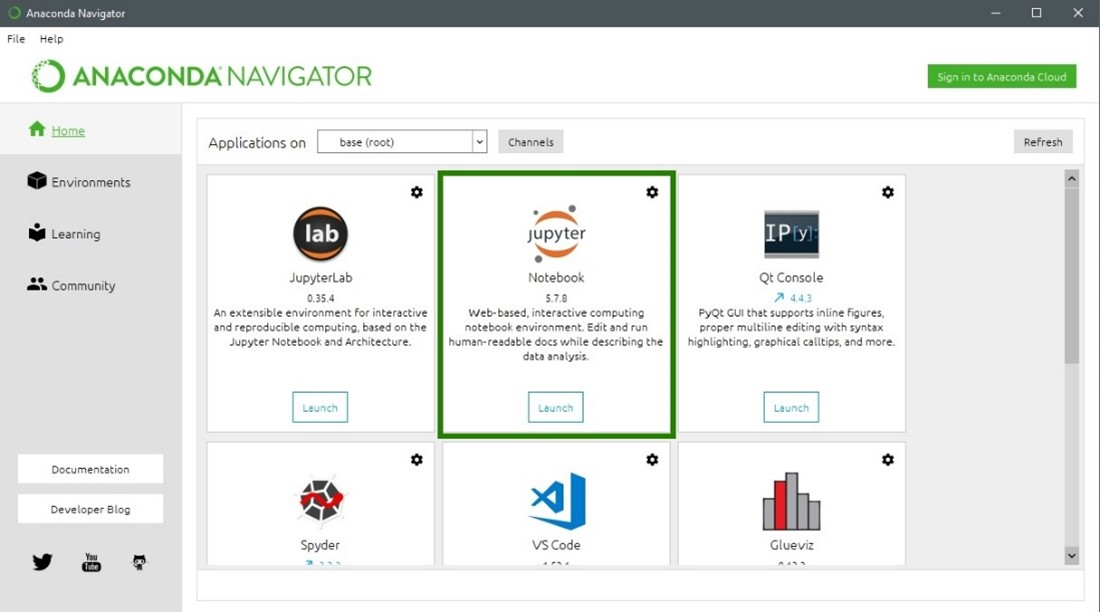
\includegraphics[width=1\textwidth]{images/anaconda.jpg}
\caption{\gls{anaconda} Navigator}
\label{fig:fig_01}
\end{figure}
\FloatBarrier

Theoretically, it would also have been possible for each developer to install \gls{anaconda} on their computer and work on the notebook, which is maintained on a \gls{GitHub} repository. However, since the project is very hardware-heavy and compiling a machine learning model can take up to several hours, a \gls{virtual machine} turns out to be the better option.

\subsection{PyCharm}
\gls{PyCharm} \cite{jetbrains_sro_pycharm_nodate} is an integrated development environment (IDE) used for programming in the Python language, created by the Czech company JetBrains. I used it because it supports anaconda, \gls{GitHub} and as a debugger.
It natively supports jupyter notebooks is perfect because it is much more comfortable than jupyter itself, then it has several extensions that make programming easier and more intuitive.

\subsection{Github}
\gls{GitHub} \cite{github_inc_github_nodate} is a provider with the function of hosting for software development and version control using Git.
Thanks to its free of charge nature it is used for most of the open-source projects.
That is why it is loved by the community of programmers, even I use it for this project to save files and use them from different locations.


\subsection{Overleaf}
\gls{Overleaf} \cite{noauthor_overleaf_nodate} is cloud-based \LaTeX{} editor, which makes writing a scientific paper collaborative. \LaTeX{} is a software widely used in the academic world to create scientific texts, with useful formatting for mathematical, statistical, computer science, physics texts, which can be problematic on other text editors.
I preferred \gls{Overleaf} to other solutions for the convenience, in fact there is no need to install anything, everything is accessible via the internet as with Colab.
\gls{Overleaf} was useful for me to write this documentation, thanks also to its versioning nature.

\subsection{MLMP}
\gls{MLMP} \cite{berner_fachhochschule_mlmp_nodate} is a cloud-based environment in which machine learning models can be trained. Similar to Colab, this environment was created by Department of Engineering and Information Technology of the Bern University of Applied Sciences (BFH), to allow its students to be able to train models, with a more performing machine. It is possible to use it in the BFH network or through a connection to the network via VPN, the advantage lies in being able to use not only the CPU, as in normal virtual machines, but also very powerful GPUs, designed precisely for this purpose.This way I can train my model much faster, having much more computing power at my disposal.

Figure~\ref{fig:fig_02} shows the available environments on \gls{MLMP}:
\begin{figure}[ht!]
\centering
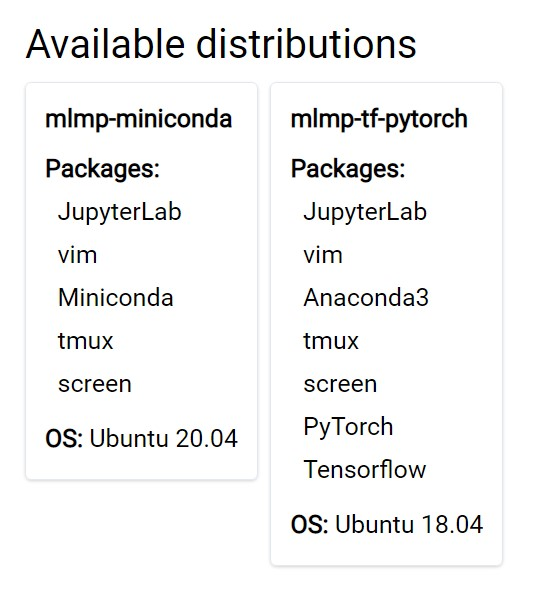
\includegraphics[width=0.5\textwidth]{images/bfhmlmp.jpg}
\caption{\gls{MLMP} distributions}
\label{fig:fig_02}
\end{figure}
\FloatBarrier
\textbf{Which distribution to use?}
To work I chose the distribution \textbf{mlmp-tf-pytorch} because it has the most suitable components for the work I need to do such as: \gls{Tensorflow} and \gls{anaconda} in full version.

As can be seen from this blog \cite{giphy_blown_nodate} the GPU takes much less time to work than the CPU.

\subsection{Scikit-learn}
Scikit-learn \cite{noauthor_scikit-learn_nodate} is a free machine learning library for Python programming language. It features various classification, regression and clustering algorithms including support vector machines, random forests, gradient boosting, k-means and DBSCAN, and is designed to interoperate with the Python numerical and scientific libraries NumPy and SciPy.

\subsection{Pandas}
\gls{Pandas} \cite{noauthor_pandas_nodate} ("Python Data Analysis Library") is an open-source library written in Python, for data analysis and data manipulation tasks.
\gls{Pandas} can be useful for example:
\begin{itemize}
    \item Convert Python lists or dictionaries, Numpy arrays, to \gls{Pandas} data frames.
    \item Inspecting data frames with a lot of functions.
    \item Data manipulation like filter, sort or group by and also data cleaning.
    \item Import local datasets that can be in different formats like CSV, TSV, Excel, etc.
    \item Access remote files or CSV databases or even websites in JSON format or read SQL tables or database.
\end{itemize}

\subsection{Tensorflow}
\gls{Tensorflow} \cite{noauthor_tensorflow_nodate} is a machine learning framework from Google, which facilitates the process of capturing data, training models, making predictions, and refining future results.

\gls{Tensorflow} is an open-source library for large-scale numerical computing and machine learning, it bundles a number of machine learning and deep learning algorithms and models.
All this is provided through the Python language; since it is easy to learn and implement. The actual mathematical operations, however, are performed in high-performance C++.

\subsection{Keras}
\gls{Keras} \cite{noauthor_keras_nodate} is an open-source software library that provides a Python interface for artificial neural networks. \gls{Keras} acts as an interface for the \gls{Tensorflow} library.

A model with \gls{Keras} consists of multiple layers, each of them performs a new data transmutation on the result from the layer above, at the end we will have a series of layers connected like a neural network.

Neural networks do not process raw data, like text files, encoded JPEG image files, or CSV files. They process vectorized and standardized representations.

For this reason, \gls{Keras} comes to our support, in fact we can use \gls{Keras} for all those tasks of data loading and data preprocessing.

Not only this, with \gls{Keras} can also perform many other tasks such as:
\begin{itemize}
    \item Build a model
    \item Train a model with the method fit()
    \item Evaluate a model
    \item Customize the method fit() for fine-tuning
\end{itemize}
See references for more details \cite{team_keras_nodate}

\subsection{BERT}
\gls{BERT} \cite{devlin_bert_2019} (Bidirectional Encoder Representations from Transformers) is an open-source deep learning model developed by Google and stat of the art for NLP tasks.

The biggest difficulty is finding the part of \gls{BERT} that suits best.
In fact, this task needed a lot of time and research to be able to figure out which \gls{BERT} is the right one for this project.

In the list below are the different versions there are of \gls{BERT}:

\begin{itemize}
    \item \gls{BERT}-Base, uncased and seven more models with trained weights released by the original \gls{BERT} authors.
    \item Small BERTs have the same general architecture but fewer and/or smaller Transformer blocks, which lets to explore tradeoffs between speed, size and quality.
    \item ALBERT \cite{lan_albert_2020}: four different sizes of "A Lite \gls{BERT}" that reduces model size (but not computation time) by sharing parameters between layers.
    \item \gls{BERT} Experts \cite{smit_chexbert_2020}: eight models that all have the \gls{BERT}-base architecture but offer a choice between different pre-training domains, to align more closely with the target task.
    \item ELECTRA \cite{clark_electra_2020} has the same architecture as \gls{BERT} (in three different sizes), but gets pre-trained as a discriminator in a set-up that resembles a Generative Adversarial Network (GAN).
    \item \gls{BERT} with Talking-Heads Attention \cite{shazeer_talking-heads_2020} and Gated GELU \cite{shazeer_glu_2020} [base, large] has two improvements to the core of the Transformer architecture.
\end{itemize}
    
\paragraph{How \gls{BERT} works?} \gls{BERT} uses Transformer, that learns contextual relations between words in a text.
Transformer is divided in two different mechanism:
\begin{itemize}
    \item encoder - that reads the text input,
    \item decoder - that produces a prediction.
\end{itemize}
The detailed workings of Transformer are described in a paper by Google \cite{vaswani_attention_2017}.

Transformer encoder reads the entire sequence of words at once. 

\paragraph{\gls{BERT} and Fine-tuning} \gls{BERT} can be used for a wide variety of language tasks, while only adding a small layer to the core model, for classification tasks like sentiment analysis one only needs to add a layer on top of the Transformer output.

\subsection{Ktrain}
\gls{Ktrain} \cite{maiya_amaiyaktrain_2021} is a lightweight wrapper open-source for the deep learning library \gls{Tensorflow} \gls{Keras}, and many pre-trained deep learning architectures like \gls{BERT}.
\gls{Ktrain} helps to build, train, and deploy neural networks and other machine learning models. 
It is designed to make deep learning and AI more accessible and easier to apply for both newcomers and experienced practitioners.

For my task, I will use the implementation of pre-trained \gls{BERT} provided by \gls{Ktrain} and fine-tune it to classify the sentiment of the reviews.


\subsection{Hugging Face}
The \gls{Hugging Face} transformers package is a very popular Python library, that provides thousands of pre-trained models for task text classification, information extraction, question answering, etc. in more than 100 languages.
Thanks to \gls{Hugging Face} NLP has become easy and accessible for everyone.
As of 2019, it also supports Tensorflow2 and not just PyTorch \cite{noauthor_pytorch_nodate} as before.
More information about Hugging Face \cite{noauthor_hugging_nodate}, the related paper \cite{wolf-etal-2020-transformers} and its source code \cite{noauthor_huggingfacetransformers_2021}.

\subsection{Plotly}
\gls{Plotly} \cite{noauthor_plotly_nodate} is a company that develops tools for creating data visualizations for data analysis.
It is also possible to have these tools online for statistical data for individuals or collaborations.
It has a library of different plots \cite{noauthor_plotly_nodate-1} and it is also possible to create dashboards thanks to \gls{Plotly} Dash \cite{noauthor_dash_nodate}.
Having Python compatible libraries was easy for me to import into my Jupyter Notebooks.